\documentclass[12pt, a4paper]{article}
\usepackage[utf8]{inputenc}
\usepackage[margin=1.2in]{geometry}
\usepackage{listings}
\usepackage{setspace}
\usepackage{xcolor}
\usepackage{titlesec}
\usepackage{enumitem}
\usepackage{amssymb}
\usepackage{amsmath}
\usepackage{tocloft}
\usepackage{bm}
\usepackage{multicol}
\usepackage{graphicx}
\graphicspath{{./Figures/}}
\usepackage{color}
\usepackage{hyperref}
\hypersetup{
	colorlinks=true,
	linkcolor=blue,
	urlcolor=blue,
	linktoc=none
}
\titleformat*{\section}{\Large\bfseries}
\titleformat*{\subsection}{\large\bfseries}
\renewcommand\thesection{\Roman{section}.}
\renewcommand\thesubsection{\alph{subsection}.}
\addtolength{\cftsecnumwidth}{16pt}

\begin{document}
\begin{spacing}{1.1}

	\begin{titlepage}
	\begin{center}
		\vspace*{1.4cm}
		
		\Huge \textbf{Capstone Project Proposal}
		
		\vspace*{1cm}
		
		
\includegraphics[scale=.5]{logo}
		
		\vspace*{1cm}
		
		\LARGE {Udacity Machine Learning Engineer Nanodegree}
		
		\vspace*{1cm}
		
		\hrule \vspace*{.5cm}
		
		\Large \textbf{A capstone proposal for analyzing worldwide food production from the years 1961-2013.}
		
		\vspace*{.5cm} \hrule
		
		\vspace*{1cm}
		
		\Large Derek Helms \\
		\Large January 13$^{th}$, 2021
	\end{center}
	\end{titlepage} \newpage

	\begin{titlepage}
		\vspace*{4cm}
		\renewcommand*\contentsname{Table of Contents}
		\tableofcontents
	\end{titlepage} \newpage

%%%% PAGE 1 %%%%

	\section{Domain Background}
	\begin{center}
	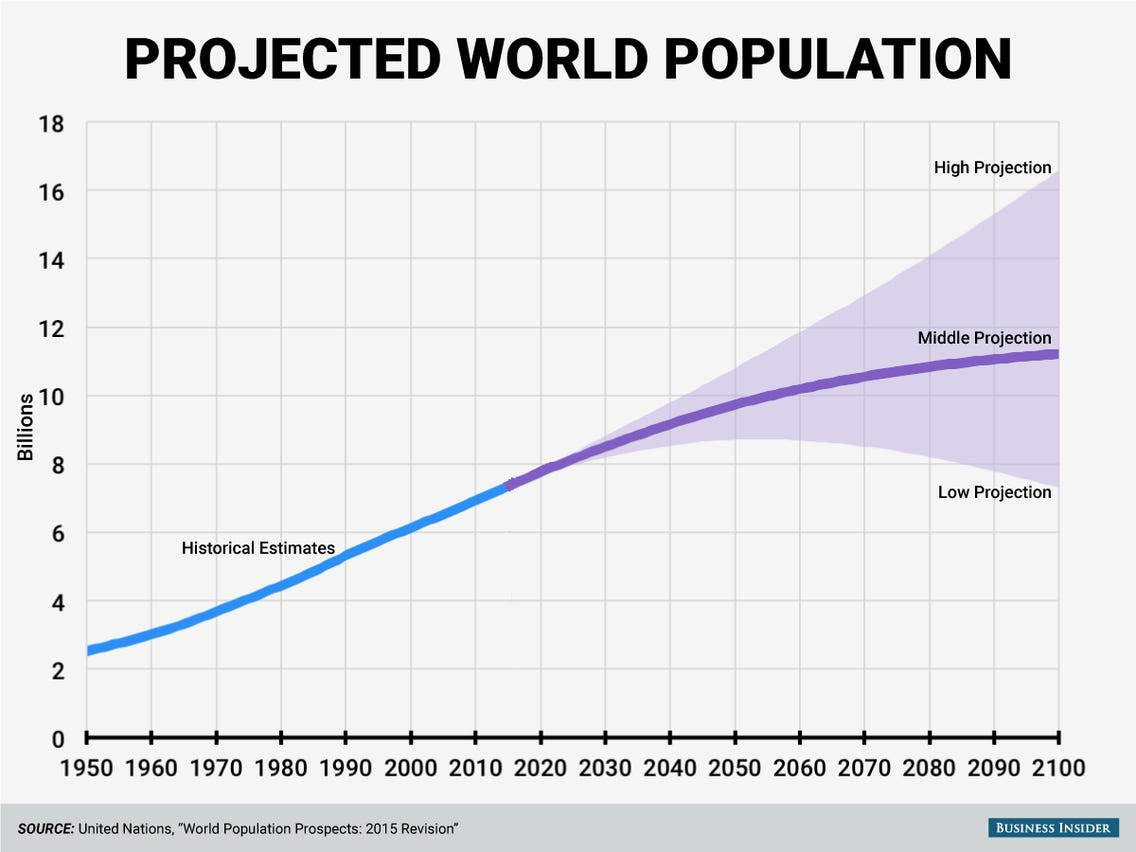
\includegraphics[scale=.24]{pop} \\
	\textit{Image obtained from source (6).}
	\end{center}
	The current world population is nearly 7.8 billion people, and this number is estimated to rise to around 9.7 billion in the year 2050. This means within the next 30 years, we will need to feed two billion more people without sacrificing the planet (1). This means we will need to double our crop production in order to feed that growing population. Agriculture is one of the greatest contributors of global warming, with farming consuming immense amounts of our water supplies and leaving major pollutants as its byproduct from fertilizer runoff (4). So how do we increase food supply without destroying our environment? \vspace*{2mm}\\
	The personal motivation for investigating this problem is my interest in applying machine learning to the field of agriculture. With an increasing need for sustainability, applying machine learning techniques to predict yield amounts or for detecting crop diseases has been a key factor in my motivation behind studying machine learning.


	\section{Problem Statement}
	With a continuously growing population this leads to the question, how do we supply the necessary amount of food for an increasing world population without sacrificing the climate of our planet? There are many solutions to this question, but the focus of this capstone will be on analyzing the global production of consumables, as well as the ratio of food (human consumption) to feed (livestock consumption) produced by each country. Only 55\% of the current world crop production is consumed by humans, with the remaining being fed to livestock. On top of this, nearly 25\% of the world's food calories are wasted before they can be consumed (4). \newpage	
	
%%%% PAGE 2 %%%%

	\section{Datasets and Inputs}
	Two different datasets will be used in the analysis, one coming from \href{https://www.kaggle.com/dorbicycle/world-foodfeed-production}{Kaggle} and one coming from \href{http://www.fao.org/faostat/en/#data/OA}{FAO} (the Food and Agriculture Organization of the United Nations).\vspace*{2mm}\\	
	The dataset obtained through Kaggle, labeled \textit{FAO\_FOOD\_STAT.csv}, is a Food Balance Sheet that originated from FAO's database, but has been formatted for easy of use, with a total of 63 features and 21477 observations. Food Balance Sheets represent the pattern of a country's food supply during a period of time, in this case it is yearly from 1961 to 2013, and measured in 1000 tonnes (2). Important features that this file contains are the country, item, element, and yearly production:
	\begin{itemize}
		\item Area: 174 unique country names from around the world.
		\item Item: 115 unique food items being globally produced.
		\item Element: food - human consumable food available at a given time. \\ 
		\hspace*{16.5mm} feed - livestock consumable food available at a given time.
		\item Y1961 - Y2013: item available at time of measurement per year.
	\end{itemize} \vspace*{2mm}
	The dataset obtained through FAO, labeled \textit{FAO\_POP.csv}, is a time series dataset that contains the estimated/projected population (for both sexes) in each country from 1961 to 2018. The estimates are based on data from the World Population Prospects and World Urbanization Prospects (3). An important note is that the population dataset contains countries and later years that are not included in the Food Balance Sheet dataset, but will be left in to account for global population and future estimates. Some important features to note within the dataset:
	\begin{itemize}
		\item Area: 245 unique country names (71 more than first dataset).
		\item Year: spans from 1961 to 2018 (5 years more than first dataset).
		\item Unit: population estimations are counted in units of 1000 persons.
		\item Value: estimate population count for each year.
	\end{itemize}\vspace*{2mm}
	The use cases for each dataset is as follows. The Kaggle dataset will be used in analyzing food production, seeing which countries produce the most and if it is for human or livestock consumption. This data will also be used to cluster countries together based on their production levels, ideally separating high and low producing countries. The FAO dataset will be used to compare the global population to the yearly total food production, as well as further analyzing the highest producing countries to see if they have the largest/fastest increasing populations. \newpage
	
%%%% PAGE 3 %%%%	
	
	\section{Solution Statement}
	As initially stated above, the problem we face is how do we produce the necessary amount of food for an exponentially increasing population without sacrificing our own planet. \vspace*{2mm}\\	
	One aspect to explore is which food items are the most produced and the use case for those food items, whether they are for human or animal consumption. This will allow us to understand where a majority of our food is being directed, and as suggested by \href{https://www.nationalgeographic.com/foodfeatures/feeding-9-billion/}{National Geographic}, could a shift in diet lead to more crops being used for human consumption rather than livestock feed. Creating graphs to find insight will allow us to see how population change has correlated to food production, and what percentage of consumables are for humans compared to livestock. \vspace*{2mm}\\	
	Another aspect of the data to explore is separating the countries into clusters based on their yearly production. Analyzing which countries are responsible for feeding the majority of the population, and how to ensure they can continue to do so. From this, we can also see which countries are not highly producing, and how we can aid them in increasing production if possible.
	
	
	\section{Benchmark Model}
	In general, the majority of this capstone will be in exploring the data and finding insights about food production through graphing and statistical methods. Creating plots for top producing country's, top produced food items, and population changes will be the main focus of the work. A large part of this will be done using Pandas, Matplotlib, and Seaborn in order to create visuals that depict trends within the two datasets. \vspace*{2mm}\\	
	We will also create a KMeans clustering model to group our data based on food production, partitioning the 174 original country's into $k$ clusters. We will want to use the \href{https://www.scikit-yb.org/en/latest/api/cluster/elbow.html}{elbow method} in selecting our number of clusters, with an initial guess of using 2 to 3 cluster to separate countries based on high and low production (and possibly medium). \vspace*{2mm}\\
	Another idea to explore will be to create a linear model that can estimate the total food production for a given year, with total population being the independent variable and total food production being the dependent varaible. This will allow us to see what the necessary production would be to support a given population number (test using the 2050 population estimate of 9.7 million).\newpage

%%%% PAGE 4 %%%%
	
	\section{Evaluation Metrics}
	With the data being unlabeled, it will be difficult to ensure that our clusters are properly partitioned. However, we can analyze both the clusters and graphs we create using two separate methods. \vspace*{2mm}\\
	One metric we can use to evaluate our model will be a \href{https://scikit-learn.org/stable/auto_examples/cluster/plot_kmeans_silhouette_analysis.html}{silhouette score}, which will measure on a scale from [-1,1] how close each point on one cluster is to points in the neighboring clusters. We will want to aim for a silhouette coefficient near +1 to indicate that our samples are far away from neighboring clusters (5). \vspace*{2mm}\\
	To evaluate our graphing and data exploration, we can use the \href{http://www.fao.org/faostat/en/#rankings/countries_by_commodity}{FAO rankings} for countries by commodity, which we can then compare to our graphs to see if we have the data correctly labeled. This ranking allows us to see the top 20 country's that produce the most for each food item, as well as the top 20 food items produced by each country from the years 1961 to 2019.	
	
	\section{Project Design}
	\textbf{1. Obtaining Data and Loading:} \\
	We will need to download data from two different sources, ensure both csv files are UTF-8 encoded, and important them to the workspace.\vspace*{2mm}\\
	\textbf{2. Data Exploration:}\\
	This is where a vast majority of the work will take place. This step includes creating graphs from subsections and groupings of the data, as well as comparing the two datasets to find insight about population and production correlation. \vspace*{2mm}\\
	\textbf{3. Data Preprocessing:}\\
	We will want to copy the original Food Balance Sheet dataset and format it in a way that can be used in our clustering algorithm. We will want to cluster based on the yearly production for each country, so dropping and filling columns necessary for that will be done in this step.\vspace*{2mm}\\
	\textbf{4. Modeling:}\\
	Here is where we will define a KMeans algorithm that will be used on the data created from step 3. We will use the elbow method in selecting our $k$ value, as well as exploring the results from our model. A possible subsection for this step would to be to explore predicting the food production for future years based on population and total yearly production using a linear model.\vspace*{2mm}\\
	\textbf{5. Conclusion:}\\
	This is where we will recap that major finding throughout the notebook and correlate it to real world problems. Any insight about the future or predictions will also be given here. \newpage
	
%%%% PAGE 5 %%%%
	
	\section{Resources}
	$[1]$ Oppenheim, Dor. ``Who Eats the Food We Grow?" \textit{Kaggle}, 30 Nov. 2017, \\ \hspace*{5mm} www.kaggle.com/dorbicycle/world-foodfeed-production. \vspace*{2.5mm}\\
	$[2]$ ``Food Balances (Old Methodology and Population)." \textit{FAOSTAT}, Food and \\ \hspace*{5mm} Agriculture Organization of the United Nations, 12 Dec. 2017, \\ \hspace*{5mm} www.fao.org/faostat/en/\#data/FBSH. \vspace*{2.5mm}\\
	$[3]$ ``Annual Population." \textit{FAOSTAT}, Food and Agriculture Organization of the \\ \hspace*{5mm} United Nations, 16 Dec. 2019, www.fao.org/faostat/en/\#data/OA. \vspace*{2.5mm}\\
	$[4]$ Foley, Jonathan. ``A Five-Step Plan to Feed the World." \textit{Feeding 9 Billion - \\ \hspace*{5mm} National Geographic}, www.nationalgeographic.com/foodfeatures/feeding-9-billion/.\vspace*{2.5mm}\\
	$[5]$ ``Selecting the Number of Clusters with Silhouette Analysis on KMeans \\ \hspace*{5mm} Clustering." \textit{Scikit}, 
	\\ \hspace*{6mm} scikit-learn.org/stable/auto\_examples/cluster/plot\_kmeans\_silhouette\_analysis.html.\vspace*{2.5mm}\\
	$[6]$ Kiersz, Andy. ``The World Could Have Another Billion People in Thirteen \\\hspace*{6mm}Years." \textit{Business Insider}, Business Insider, 29 July 2015,\\\hspace*{6mm}www.businessinsider.com/un-world-population-projections-2015-7. \vspace*{2.5mm}\\
	
	
	
\end{spacing}
\end{document}